


\tikzset{every picture/.style={line width=0.75pt}} %set default line width to 0.75pt        

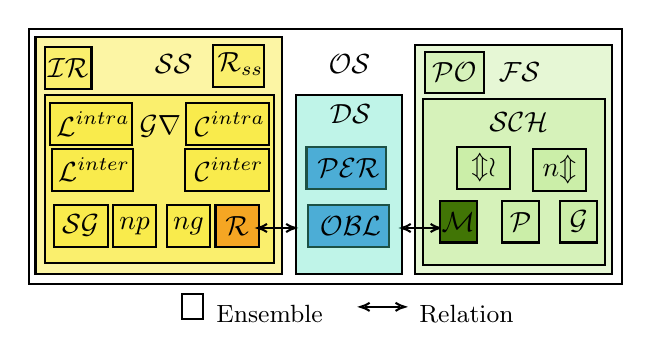
\begin{tikzpicture}[x=0.75pt,y=0.75pt,yscale=-1,xscale=1]
    %uncomment if require: \path (0,2639); %set diagram left start at 0, and has height of 2639

    %Shape: Rectangle [id:dp3362927554270163] 
    \draw  [fill={rgb, 255:red, 255; green, 255; blue, 255 }  ,fill opacity=1 ] (110,850) -- (396,850) -- (396,973) -- (110,973) -- cycle ;
    %Shape: Rectangle [id:dp9693207675537321] 
    \draw  [fill={rgb, 255:red, 184; green, 233; blue, 134 }  ,fill opacity=0.34 ] (296,858) -- (391.1,858) -- (391.1,968) -- (296,968) -- cycle ;
    %Shape: Rectangle [id:dp44516812254176785] 
    \draw  [fill={rgb, 255:red, 184; green, 233; blue, 134 }  ,fill opacity=0.34 ] (300,884) -- (387.83,884) -- (387.83,964) -- (300,964) -- cycle ;
    %Shape: Rectangle [id:dp6429506751223992] 
    \draw  [fill={rgb, 255:red, 248; green, 231; blue, 28 }  ,fill opacity=0.4 ] (113.27,854) -- (232,854) -- (232,968) -- (113.27,968) -- cycle ;
    %Straight Lines [id:da4994570811739021] 
    \draw    (291.69,946) -- (306,946) ;
    \draw [shift={(308,946)}, rotate = 180] [color={rgb, 255:red, 0; green, 0; blue, 0 }  ][line width=0.75]    (4.37,-1.96) .. controls (2.78,-0.92) and (1.32,-0.27) .. (0,0) .. controls (1.32,0.27) and (2.78,0.92) .. (4.37,1.96)   ;
    \draw [shift={(289.69,946)}, rotate = 0] [color={rgb, 255:red, 0; green, 0; blue, 0 }  ][line width=0.75]    (4.37,-1.96) .. controls (2.78,-0.92) and (1.32,-0.27) .. (0,0) .. controls (1.32,0.27) and (2.78,0.92) .. (4.37,1.96)   ;
    %Shape: Rectangle [id:dp12404915901017843] 
    \draw  [fill={rgb, 255:red, 248; green, 231; blue, 28 }  ,fill opacity=0.4 ] (117.81,882) -- (228,882) -- (228,963) -- (117.81,963) -- cycle ;
    %Shape: Rectangle [id:dp011814159340156172] 
    \draw  [fill={rgb, 255:red, 248; green, 231; blue, 28 }  ,fill opacity=0.4 ] (150.59,935) -- (171.41,935) -- (171.41,955) -- (150.59,955) -- cycle ;

    %Shape: Rectangle [id:dp6366814864369554] 
    \draw  [fill={rgb, 255:red, 248; green, 231; blue, 28 }  ,fill opacity=0.4 ] (122,935) -- (148,935) -- (148,955) -- (122,955) -- cycle ;
    %Shape: Rectangle [id:dp4224844209889693] 
    \draw  [fill={rgb, 255:red, 248; green, 231; blue, 28 }  ,fill opacity=0.4 ] (121.02,908) -- (160.03,908) -- (160.03,928) -- (121.02,928) -- cycle ;

    %Shape: Rectangle [id:dp2109151755211085] 
    \draw  [fill={rgb, 255:red, 248; green, 231; blue, 28 }  ,fill opacity=0.4 ] (120.22,886) -- (159.8,886) -- (159.8,906) -- (120.22,906) -- cycle ;

    %Shape: Rectangle [id:dp5612046560441226] 
    \draw  [fill={rgb, 255:red, 248; green, 231; blue, 28 }  ,fill opacity=0.4 ] (185.83,886) -- (225.95,886) -- (225.95,906) -- (185.83,906) -- cycle ;

    %Shape: Rectangle [id:dp8653779879037786] 
    \draw  [fill={rgb, 255:red, 248; green, 231; blue, 28 }  ,fill opacity=0.4 ] (185.29,908) -- (225.72,908) -- (225.72,928) -- (185.29,928) -- cycle ;

    %Shape: Rectangle [id:dp5118226471482248] 
    \draw  [fill={rgb, 255:red, 65; green, 117; blue, 5 }  ,fill opacity=1 ] (308.01,933) -- (325.99,933) -- (325.99,953) -- (308.01,953) -- cycle ;

    %Shape: Rectangle [id:dp9933924068366515] 
    \draw  [fill={rgb, 255:red, 248; green, 231; blue, 28 }  ,fill opacity=0.4 ] (176.63,935) -- (197.37,935) -- (197.37,955) -- (176.63,955) -- cycle ;

    %Shape: Rectangle [id:dp8500726713846194] 
    \draw  [fill={rgb, 255:red, 248; green, 231; blue, 28 }  ,fill opacity=0.4 ] (117.75,859) -- (140.25,859) -- (140.25,879) -- (117.75,879) -- cycle ;

    %Shape: Rectangle [id:dp5924732056565294] 
    \draw  [fill={rgb, 255:red, 248; green, 231; blue, 28 }  ,fill opacity=0.4 ] (198.98,858) -- (223.16,858) -- (223.16,878) -- (198.98,878) -- cycle ;

    %Shape: Rectangle [id:dp346383687870204] 
    \draw  [fill={rgb, 255:red, 74; green, 144; blue, 226 }  ,fill opacity=1 ] (243.84,907) -- (282.24,907) -- (282.24,927) -- (243.84,927) -- cycle ;

    %Shape: Rectangle [id:dp8336033635496647] 
    \draw  [fill={rgb, 255:red, 74; green, 144; blue, 226 }  ,fill opacity=1 ] (244.57,935) -- (283.48,935) -- (283.48,955) -- (244.57,955) -- cycle ;

    %Shape: Rectangle [id:dp7738606236066947] 
    \draw  [fill={rgb, 255:red, 184; green, 233; blue, 134 }  ,fill opacity=0.34 ] (300.75,861) -- (329.25,861) -- (329.25,881) -- (300.75,881) -- cycle ;

    %Shape: Rectangle [id:dp7635846319928088] 
    \draw  [fill={rgb, 255:red, 184; green, 233; blue, 134 }  ,fill opacity=0.34 ] (316.43,907) -- (342,907) -- (342,927) -- (316.43,927) -- cycle ;

    %Shape: Rectangle [id:dp3026483542328955] 
    \draw  [fill={rgb, 255:red, 184; green, 233; blue, 134 }  ,fill opacity=0.34 ] (353.11,908) -- (378.29,908) -- (378.29,928) -- (353.11,928) -- cycle ;

    %Shape: Rectangle [id:dp8981167883687693] 
    \draw  [fill={rgb, 255:red, 184; green, 233; blue, 134 }  ,fill opacity=0.34 ] (366.02,933) -- (384,933) -- (384,953) -- (366.02,953) -- cycle ;

    %Shape: Rectangle [id:dp9543580464730599] 
    \draw  [fill={rgb, 255:red, 184; green, 233; blue, 134 }  ,fill opacity=0.34 ] (338,933) -- (355.98,933) -- (355.98,953) -- (338,953) -- cycle ;

    %Shape: Rectangle [id:dp9228172603845481] 
    \draw  [fill={rgb, 255:red, 245; green, 166; blue, 35 }  ,fill opacity=1 ] (200,935) -- (220.77,935) -- (220.77,955) -- (200,955) -- cycle ;

    %Shape: Rectangle [id:dp07186794284626385] 
    \draw  [fill={rgb, 255:red, 255; green, 255; blue, 255 }  ,fill opacity=1 ] (184,978) -- (193.81,978) -- (193.81,990) -- (184,990) -- cycle ;
    %Straight Lines [id:da11132308874086716] 
    \draw    (271.87,984) -- (277.73,984) -- (289.12,984) ;
    \draw [shift={(291.12,984)}, rotate = 180] [color={rgb, 255:red, 0; green, 0; blue, 0 }  ][line width=0.75]    (4.37,-1.96) .. controls (2.78,-0.92) and (1.32,-0.27) .. (0,0) .. controls (1.32,0.27) and (2.78,0.92) .. (4.37,1.96)   ;
    \draw [shift={(269.87,984)}, rotate = 0] [color={rgb, 255:red, 0; green, 0; blue, 0 }  ][line width=0.75]    (4.37,-1.96) .. controls (2.78,-0.92) and (1.32,-0.27) .. (0,0) .. controls (1.32,0.27) and (2.78,0.92) .. (4.37,1.96)   ;
    %Straight Lines [id:da3653401525747466] 
    \draw    (236.4,946) -- (222.42,946) ;
    \draw [shift={(220.42,946)}, rotate = 360] [color={rgb, 255:red, 0; green, 0; blue, 0 }  ][line width=0.75]    (4.37,-1.96) .. controls (2.78,-0.92) and (1.32,-0.27) .. (0,0) .. controls (1.32,0.27) and (2.78,0.92) .. (4.37,1.96)   ;
    \draw [shift={(238.4,946)}, rotate = 180] [color={rgb, 255:red, 0; green, 0; blue, 0 }  ][line width=0.75]    (4.37,-1.96) .. controls (2.78,-0.92) and (1.32,-0.27) .. (0,0) .. controls (1.32,0.27) and (2.78,0.92) .. (4.37,1.96)   ;
    %Shape: Rectangle [id:dp5768315579377827] 
    \draw  [fill={rgb, 255:red, 80; green, 227; blue, 194 }  ,fill opacity=0.36 ] (238.57,882) -- (290,882) -- (290,968) -- (238.57,968) -- cycle ;


    % Text Node
    \draw (318,985) node  [font=\footnotesize] [align=left] {\begin{minipage}[lt]{29.67pt}\setlength\topsep{0pt}
            \begin{center}
                {\small Relation}
            \end{center}

        \end{minipage}};
    % Text Node
    \draw (224,985) node  [font=\footnotesize] [align=left] {\begin{minipage}[lt]{35.37pt}\setlength\topsep{0pt}
            \begin{center}
                {\small Ensemble}
            \end{center}

        \end{minipage}};
    % Text Node
    \draw (264.5,867) node   [align=left] {$\displaystyle \mathcal{OS}$};
    % Text Node
    \draw (135,945) node   [align=left] {$\displaystyle \mathcal{SG}$};
    % Text Node
    \draw (265,891) node   [align=left] {$\displaystyle \mathcal{DS}$};
    % Text Node
    \draw (179.87,867) node   [align=left] {$\displaystyle \mathcal{SS}$};
    % Text Node
    \draw (173.38,897) node   [align=left] {$\displaystyle \mathcal{Gr}$};
    % Text Node
    \draw (346.5,871) node   [align=left] {$\displaystyle \mathcal{FS}$};
    % Text Node
    \draw (346.04,895) node   [align=left] {$\displaystyle \mathcal{SCH}$};
    % Text Node
    \draw (210.38,945) node   [align=left] {$\displaystyle \mathcal{R}$};
    % Text Node
    \draw (346.99,943) node   [align=left] {$\displaystyle \mathcal{P}$};
    % Text Node
    \draw (375.01,943) node   [align=left] {$\displaystyle \mathcal{G}$};
    % Text Node
    \draw (365.7,918) node   [align=left] {$\displaystyle n\mathcal{m}$};
    % Text Node
    \draw (329.21,917) node   [align=left] {$\displaystyle \mathcal{mo}$};
    % Text Node
    \draw (315,871) node   [align=left] {$\displaystyle \mathcal{PO}$};
    % Text Node
    \draw (265,945) node   [align=left] {$\displaystyle \mathcal{OBL}$};
    % Text Node
    \draw (264,917) node   [align=left] {$\displaystyle \mathcal{PER}$};
    % Text Node
    \draw (212,867) node   [align=left] {$\displaystyle \mathcal{R}_{ss}$};
    % Text Node
    \draw (129,869) node   [align=left] {$\displaystyle \mathcal{IR}$};
    % Text Node
    \draw (187,945) node   [align=left] {$\displaystyle \mathnormal{ng}$};
    % Text Node
    \draw (317,943) node   [align=left] {$\displaystyle \mathcal{M}$};
    % Text Node
    \draw (206.51,918) node   [align=left] {$\displaystyle \mathcal{C}^{inter}$};
    % Text Node
    \draw (206.89,896) node   [align=left] {$\displaystyle \mathcal{C}^{intra}$};
    % Text Node
    \draw (141,896) node   [align=left] {$\displaystyle \mathcal{L}^{intra}$};
    % Text Node
    \draw (141.5,918) node   [align=left] {$\displaystyle \mathcal{L}^{inter}$};
    % Text Node
    \draw (161,945) node   [align=left] {$\displaystyle \mathnormal{np}$};


\end{tikzpicture}